%%%%%%%%%%%%%%%%%%%%%%%%%%%%%%%%%%%%%%%%%%%%%%%%%%%%%%%%%%%
% --------------------------------------------------------
% Tau
% LaTeX Template
% Version 2.4.4 (28/02/2025)
%
% Author: 
% Guillermo Jimenez (memo.notess1@gmail.com)
% 
% License:
% Creative Commons CC BY 4.0
% --------------------------------------------------------
%%%%%%%%%%%%%%%%%%%%%%%%%%%%%%%%%%%%%%%%%%%%%%%%%%%%%%%%%%%

\documentclass[9pt,a4paper,column,twoside]{tau-class/tau}
\usepackage[english]{babel}
\usepackage{graphicx}
\usepackage{amsmath}
\usepackage{subcaption}

%% Spanish babel recomendation
% \usepackage[spanish,es-nodecimaldot,es-noindentfirst]{babel} 

%% Draft watermark
% \usepackage{draftwatermark}

%----------------------------------------------------------
% TITLE
%----------------------------------------------------------

\journalname{Intro Microelectronic Circuits with Laboratory}
\title{Resistors and Diodes}

%----------------------------------------------------------
% AUTHORS, AFFILIATIONS AND PROFESSOR
%----------------------------------------------------------

\author[1]{Henry Tejada Deras}
\author[1]{Anika Mahesh}
\author[1]{Elias Tuthill}

%----------------------------------------------------------

\affil[1]{Franklin W. Olin College of Engineering}

%----------------------------------------------------------
% FOOTER INFORMATION
%----------------------------------------------------------

\institution{Franklin W. Olin College of Engineering}
\footinfo{Intro Microelectronic Circuits with Laboratory}
\theday{April 22, 2026}
\leadauthor{Tejada Deras et al.}

%----------------------------------------------------------

\begin{document}
		
    \maketitle 
    \thispagestyle{firststyle} 
    % \tauabstract 
    % \tableofcontents
    % \linenumbers 
    
%----------------------------------------------------------

\section{Experiment 1: Diode-Connected Transistor Characteristics}
\subsection{Results}
\begin{figure}[H]
    \centering
    \begin{subfigure}{0.46\linewidth}
        \centering
        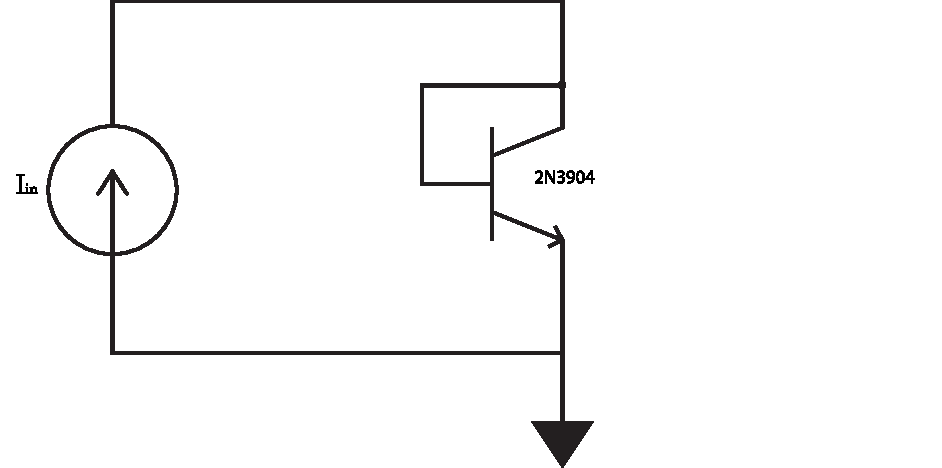
\includegraphics[width=\linewidth]{../diagrams/lab2_circuit1.pdf}
        \caption{Current source circuit.}\label{fig:diagram1a}
    \end{subfigure}
    \hfill
    \begin{subfigure}{0.53\linewidth}
        \centering
        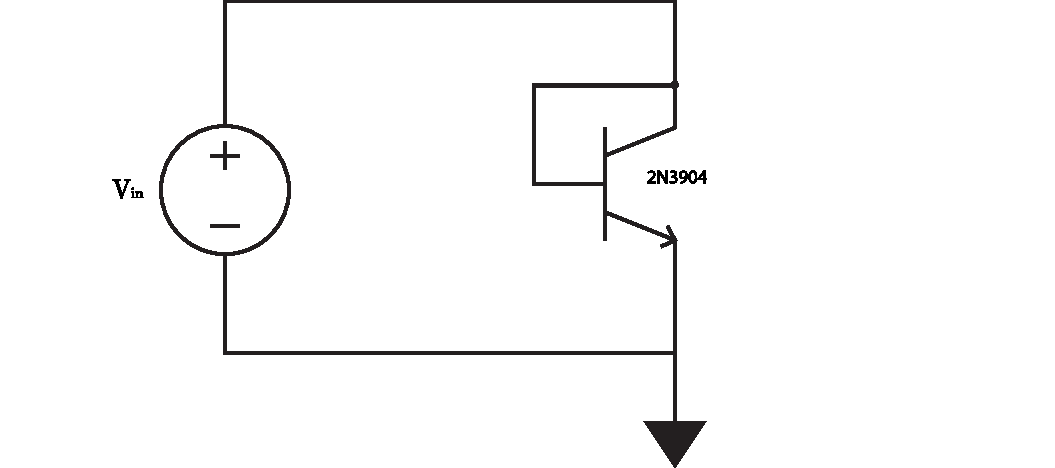
\includegraphics[width=\linewidth]{../diagrams/lab2_circuit2.pdf}
        \caption{Voltage source circuit.}\label{fig:diagram1b}
    \end{subfigure}
    \caption{The schematic for the experimental setups used in Experiment 1.}
    \label{fig:diagram1}
\end{figure}
% Make a single semilog plot for your report showing the voltage–current characterisitc, the current–voltage characteristic, and the theoretical fit, and the extracted parameters.
    From the voltage data and the current data, we can plot the voltage–current characteristic and the current–voltage characteristic of the diode-connected transistor, along with a theoretical fit to the data. The theoretical fit is based on the exponential model of a diode, which can be expressed as:
	\begin{itemize}
		\item Fitted Line Equation when voltage was sourced and current was measured: $\text{y = }e^{(41.56 \Omega)\text{x} - 34.51 \text{V}}$
		\item Fitted Line Equation when current was sourced and voltage was measured: $\text{y = }e^{(39.46 \Omega)\text{x} - 33.46 \text{V}}$
	\end{itemize}
    \begin{figure}[H]
        \centering
        \includegraphics[width=0.7\linewidth]{../diagrams/lab2_exp1_plt1.pdf}
        \caption{The voltage–current characteristic, the current–voltage characteristic, and the theoretical fit for the diode-connected transistor.}\label{fig:exp1_plot}
    \end{figure} 
    By taking the derivative of the voltage with respect to the current using numerical differentiation techniques, we can find the incremental resistance of the diode-connected transistor as a function of the current flowing through it. The incremental resistance can be expressed as $r_d = \frac{U_t}{I}$ where $U_t = 0.0191$ V as estimated by the fitted line.\\
    \begin{figure}[H]
        \centering
        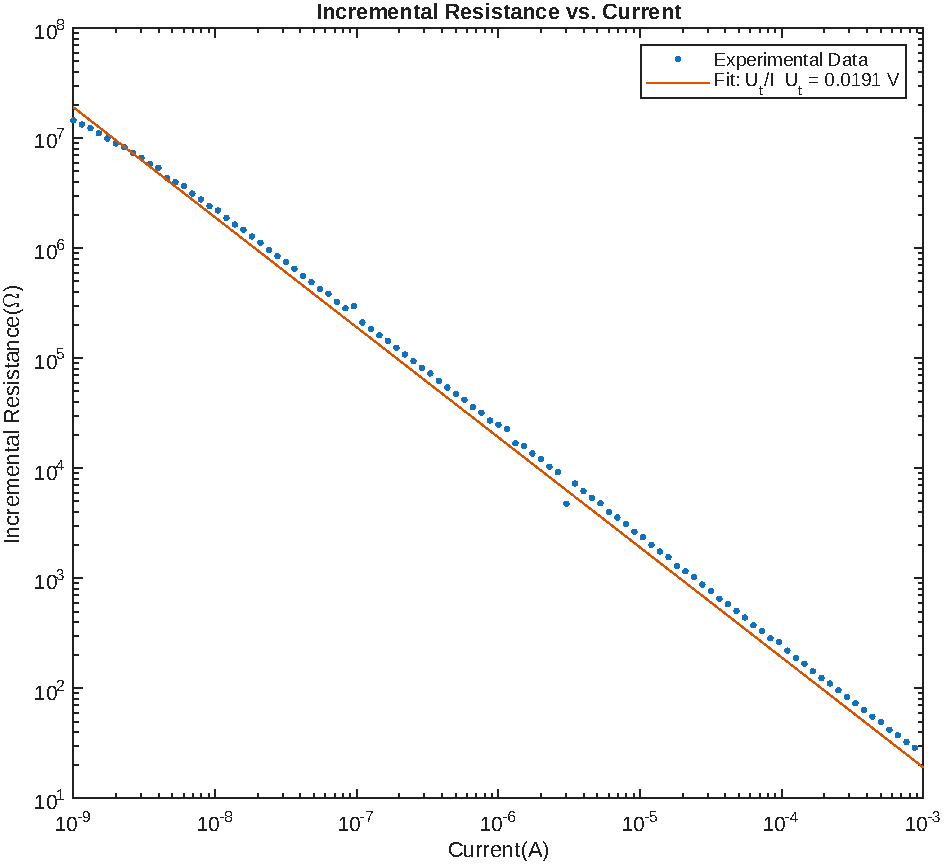
\includegraphics[width=0.7\linewidth]{../diagrams/lab2_exp1_plt2.pdf}
        \caption{A log-log plot showing the incremental resistance of the diode-connected transistor as a function of the current flowing through it, along with a theoretical fit to the data.}\label{fig:exp1_plot}
    \end{figure} 
	% For your report, make a log-log plot showing the incremental resistance of your diode-connected transistor as a function of the current flowing through it, along with a theoretical fit to the data. Does the theoretical fit match the data?
	\subsection{Analysis}
    The voltage–current characteristic and the current–voltage characteristic should ideally be the same. And this shows in the line of best fits where the differences are marginal. However, due to some measurement errors and the non-ideal behavior of the diode, the lines of best fit are not identical. The theoretical fits match the data reasonably well, especially in the region where the diode is forward-biased. However, there are deviations from the theoretical fit at low currents due to leakage currents. This can be accounted for by not using low current data points when fitting the exponential model. \\ \\
    The incremental resistance of the diode-connected transistor decreases as current increases as they are inversely proportional. The theoretical fit for the incremental resistance matches the data well at higher currents. however, at lower currents, the fit does not match the data accurately due to the presence of leakage currents and the non-ideal behavior of the diode at low currents.
	\subsection{Discussion}
    The measured characteristics of the diode-connected transistor 
    follows the expected exponential relationship between current and voltage. 
    Over multiple decades of current, the semilog plot in Fig.~\ref{fig:exp1_semilog} looks mostly linear,
    which is consistent with the ideal diode equation
    \[
    I = I_s(e^{V/U_T} - 1)
    \] The thermal voltage found from the exponential fit was $U_T = 0.0191$ V. This is slightly lower than the typical room
    temperature of about 25-26mV, but still in the correct order of magnitude. This slight variation could be caused by instrumentation resolution,
    noise, or some temperature variation. \\ \\
    Overall, the experimental results show that the diode-connected transistor behaves similarly
    to an ideal diode over a wide range of currents. While some deviations show up at very low current levels,
    the exponential model provides a reasonable approximation of behavior within the forward-bias region.
\section{Experiment 2: Characteristics of a Resistor and Diode in Series}
	\subsection{Results}
	\begin{figure}[H]
 		\centering
   		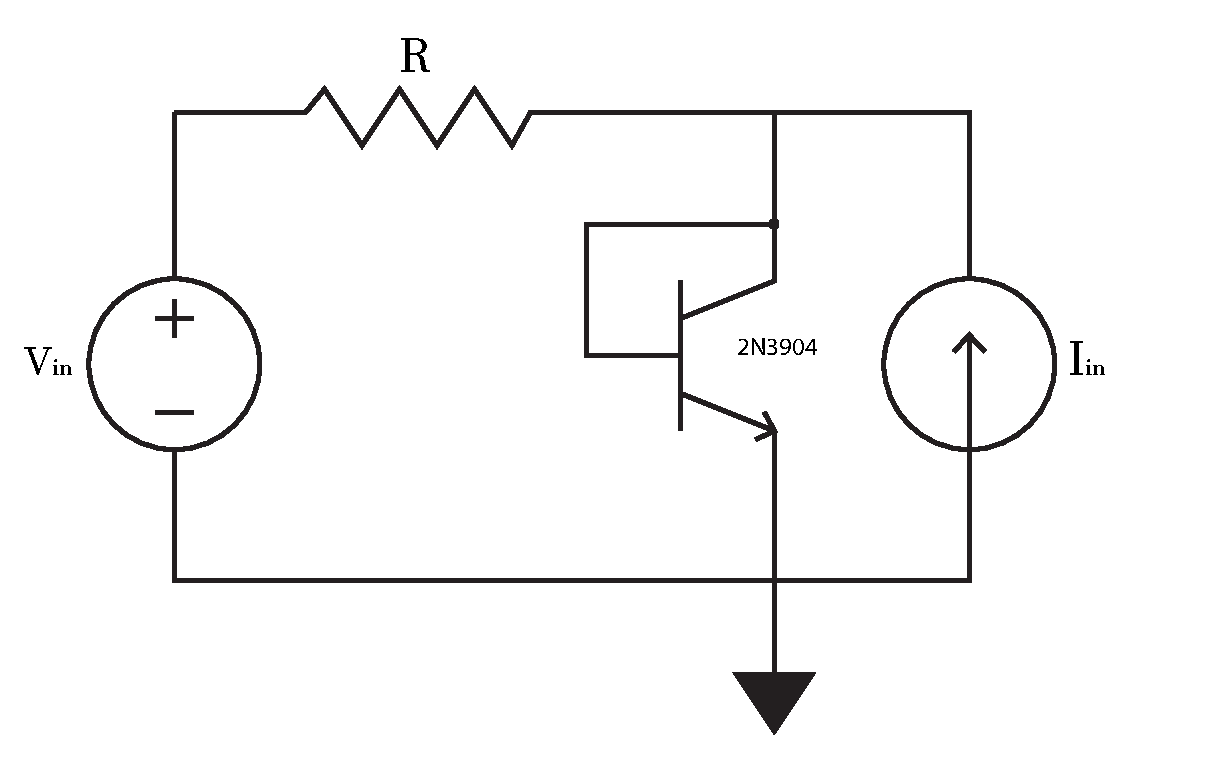
\includegraphics[width=0.7\linewidth]{../diagrams/lab2_circuit3.pdf}
   		\caption{The schematic for the experimental setups used in Experiment 2.}\label{fig:exp2_diag}
    \end{figure}
    \begin{figure}[H]
        \centering
        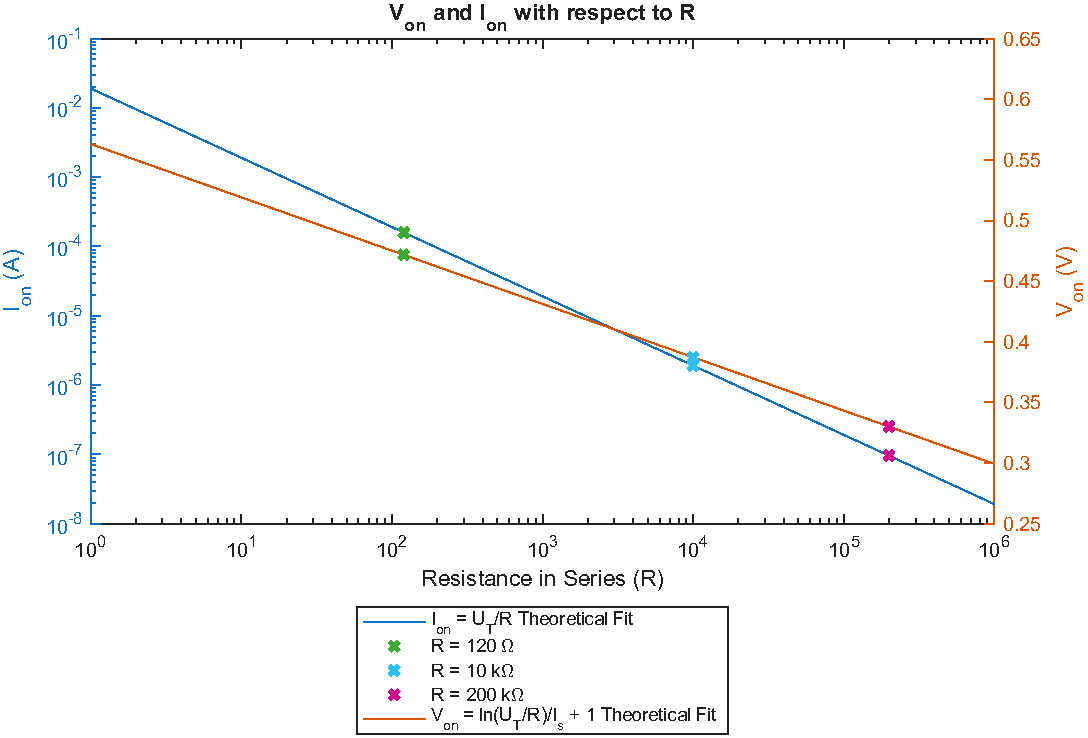
\includegraphics[width=0.7\linewidth]{../diagrams/lab2_exp2_V_on,_I_on_with_respect_to_R.pdf}
        \caption{The measured values of $I_{on}$ and $V_{on}$ match the predicted values from the relationship derived in the prelab.}\label{fig:v_on,i_on_respect_r}
    \end{figure}
    The measured values of $V_{on}$ and $I_{on}$ fit in the theoretical plots. They vary as we expected based on a change of resistance, $R$.
    \begin{figure}[H]
        \centering
        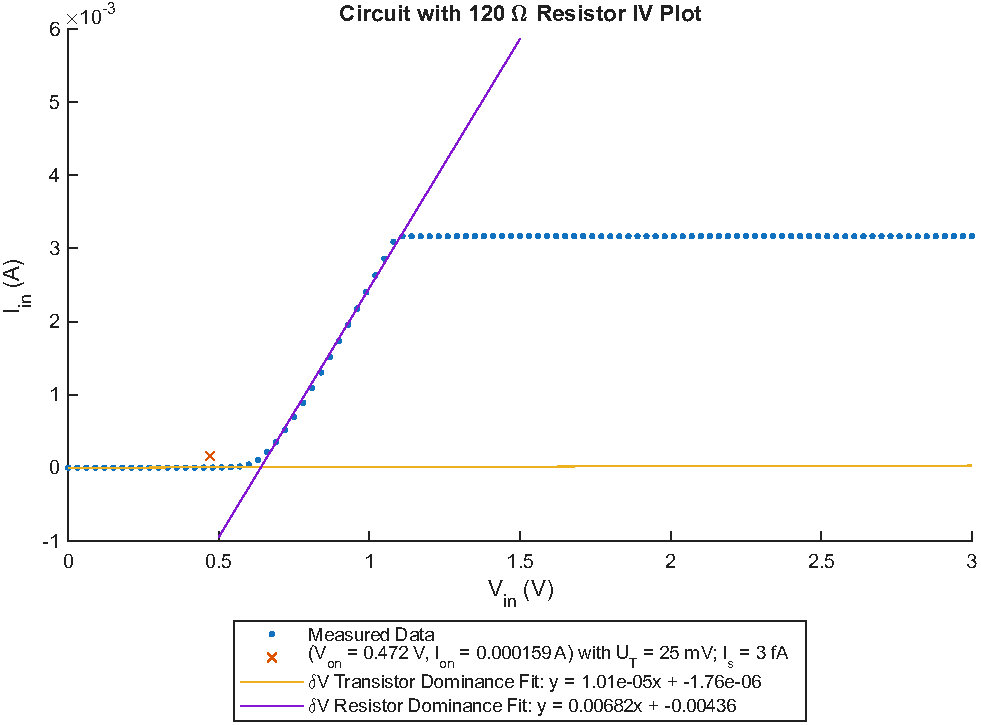
\includegraphics[width=0.7\linewidth]{../diagrams/lab2_exp2_V_in_vs_I_in_120Ohm.pdf}
        \caption{Input voltage vs input current for a 120~$\Omega$ load.}\label{fig:vin_vs_iin_120Ohm}
    \end{figure}

    \begin{figure}[H]
        \centering
        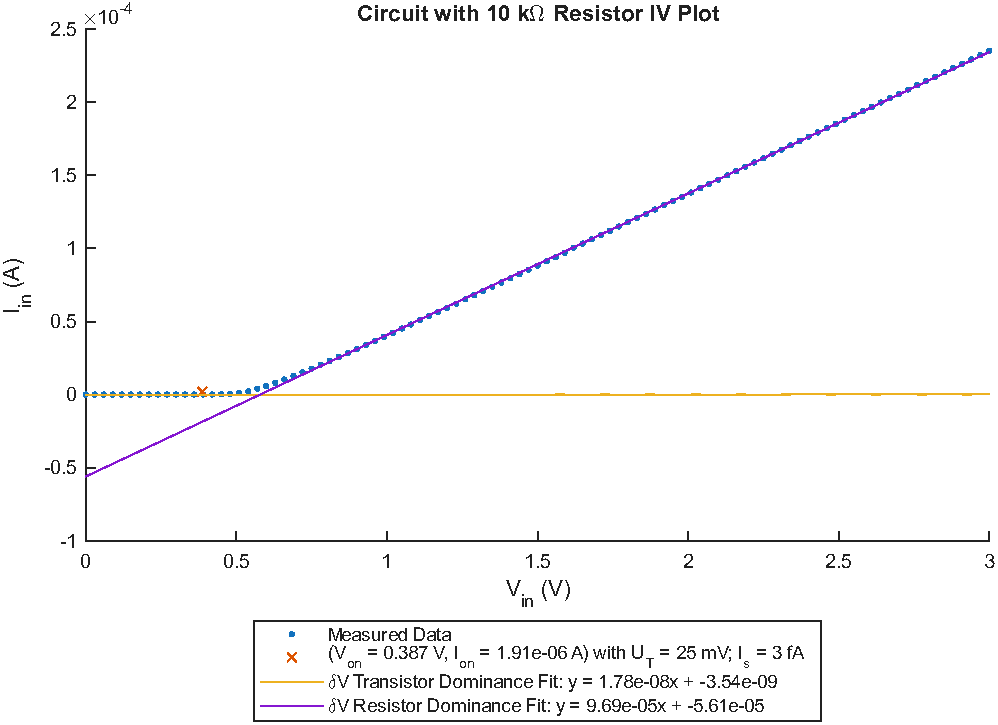
\includegraphics[width=0.7\linewidth]{../diagrams/lab2_exp2_V_in_vs_I_in_10kOhm.pdf}
        \caption{Input voltage vs input current for a 10~k$\Omega$ load.}\label{fig:vin_vs_iin_10kOhm}
    \end{figure}

    \begin{figure}[H]
        \centering
        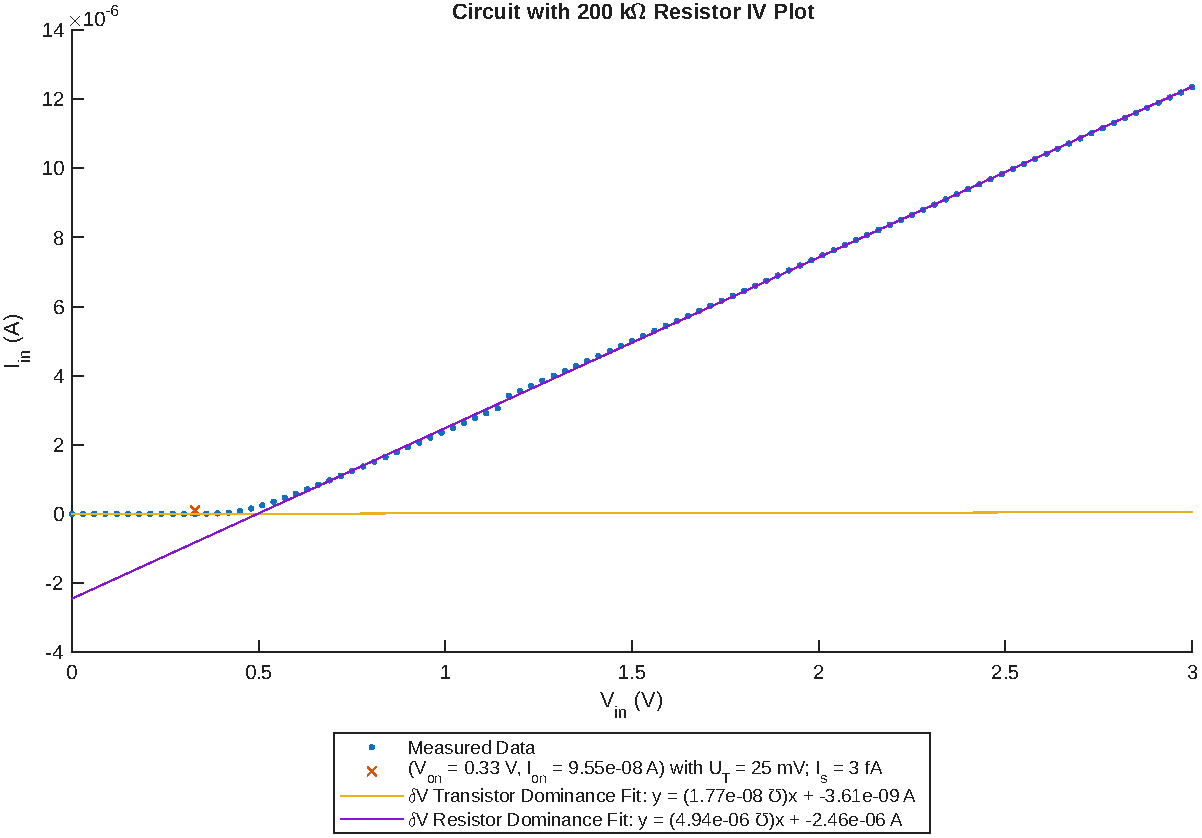
\includegraphics[width=0.7\linewidth]{../diagrams/lab2_exp2_V_in_vs_I_in_200kOhm.pdf}
        \caption{Input voltage vs input current for a 200~k$\Omega$ load.}\label{fig:vin_vs_iin_200kOhm}
    \end{figure}
    The two regimes of operation are apparent as predicted through the equations derived from the prelab. The equations accurately describe how the change in voltage across the resistor dominates after the $(V_{on}, I_{on})$ point and the change in voltage across the transistor dominates earlier. As you can see from the plots, each one contains both regimes and are both separated by whether the $(V_{on}, I_{on})$ point has been passed.

    \begin{figure}[H]
        \centering
        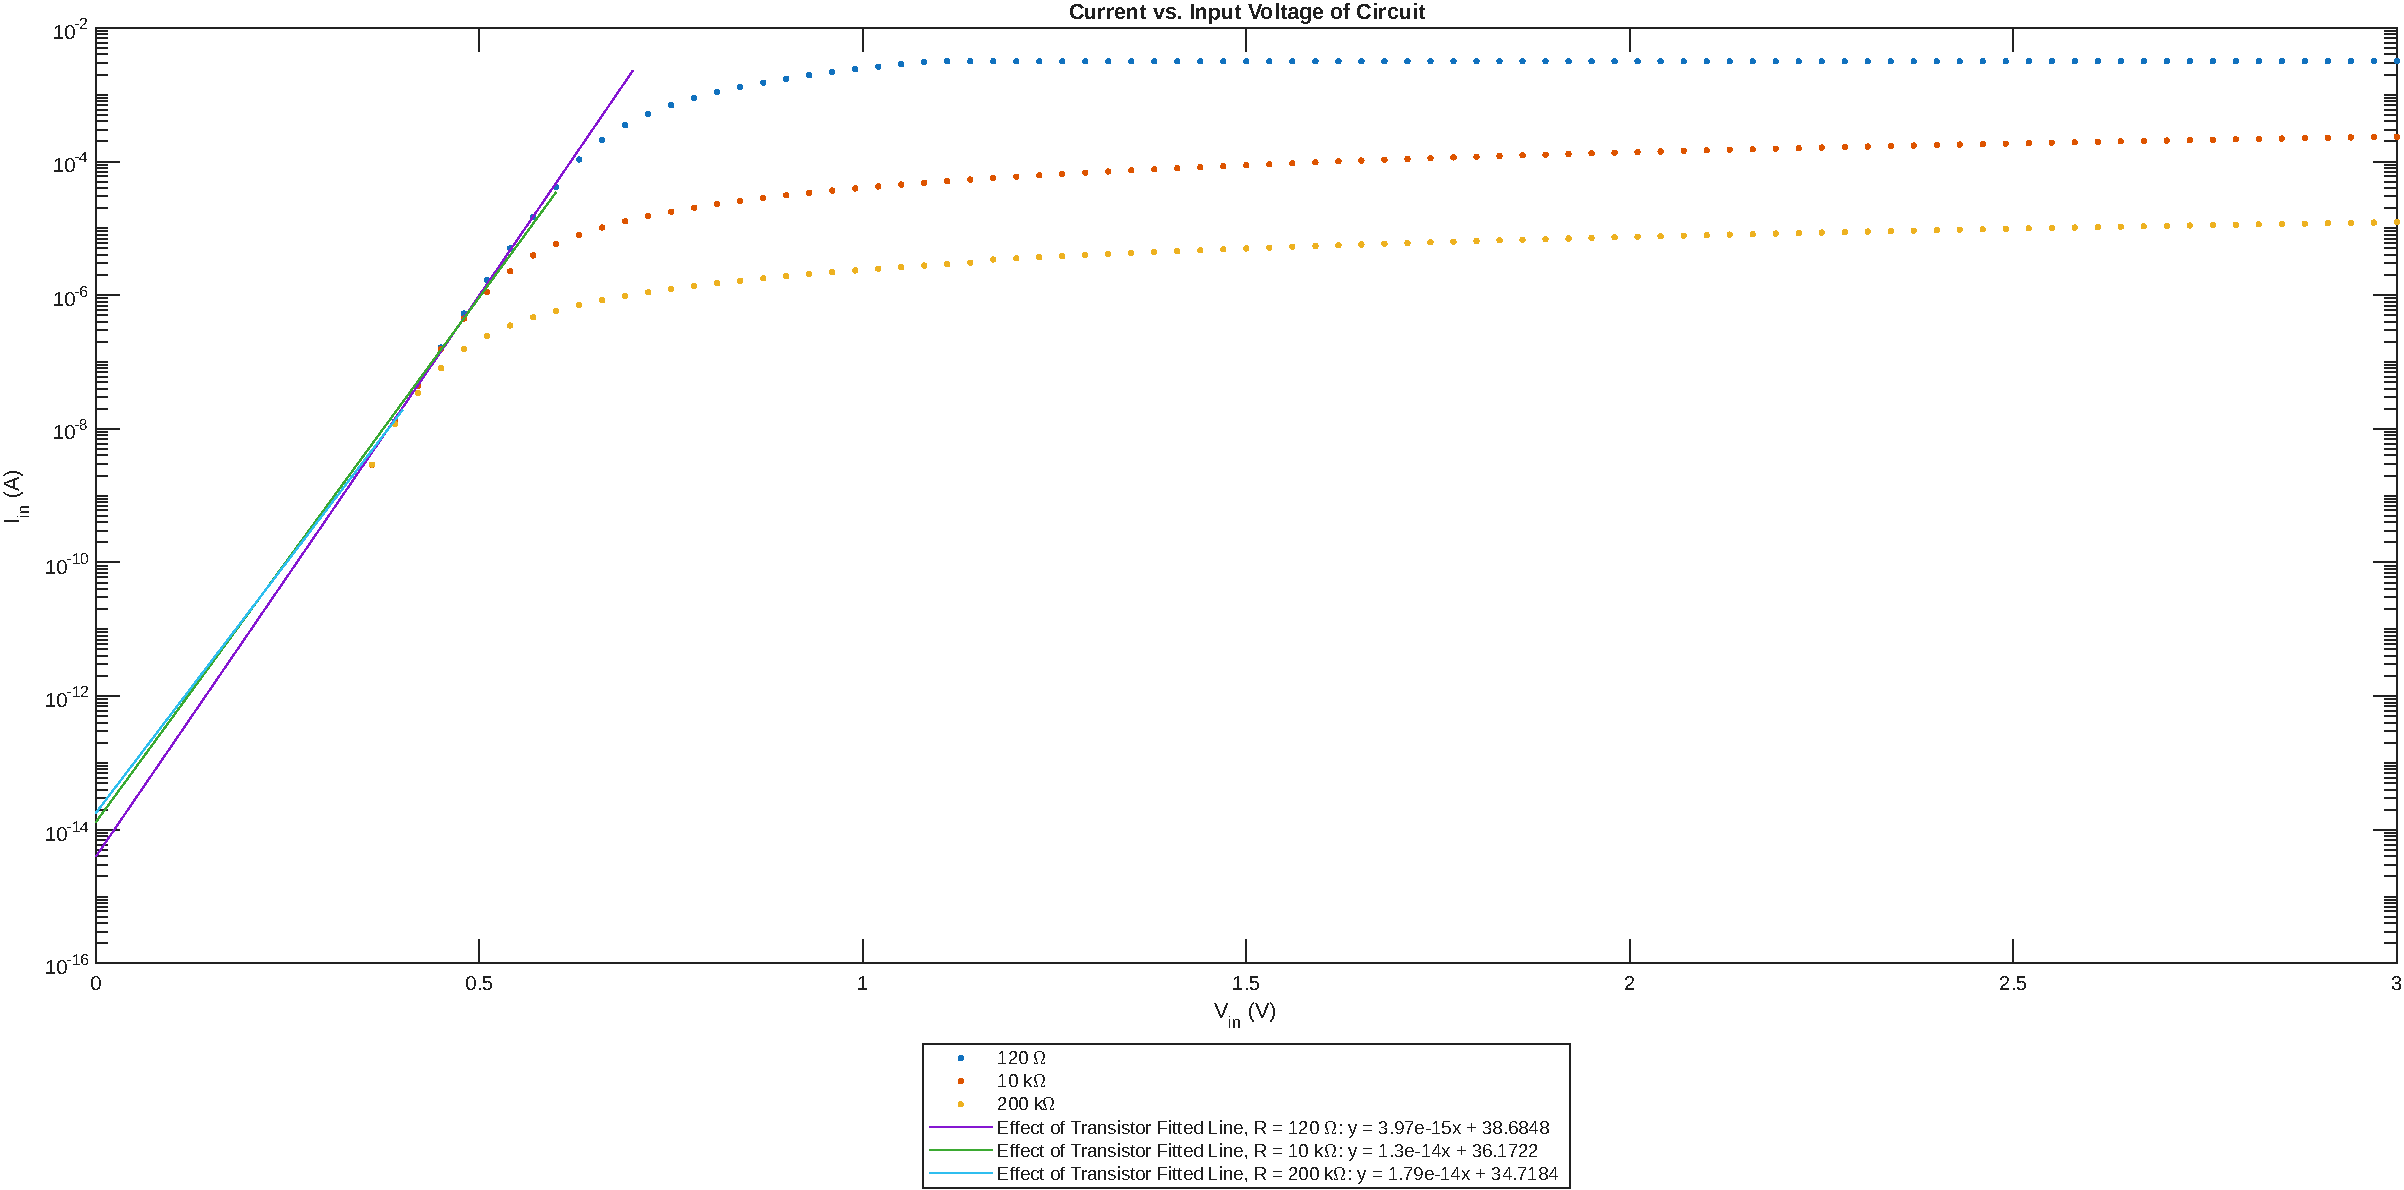
\includegraphics[width=0.7\linewidth]{../diagrams/lab2_exp2_V_in_vs_I_in.pdf}
        \caption{Input current to the circuit with respect to the input voltage to the circuit. The relationship matches the theoretical.}\label{fig:circuit_i_in_vs_v_in}
    \end{figure}
    The 
    \begin{figure}[H]
        \centering
        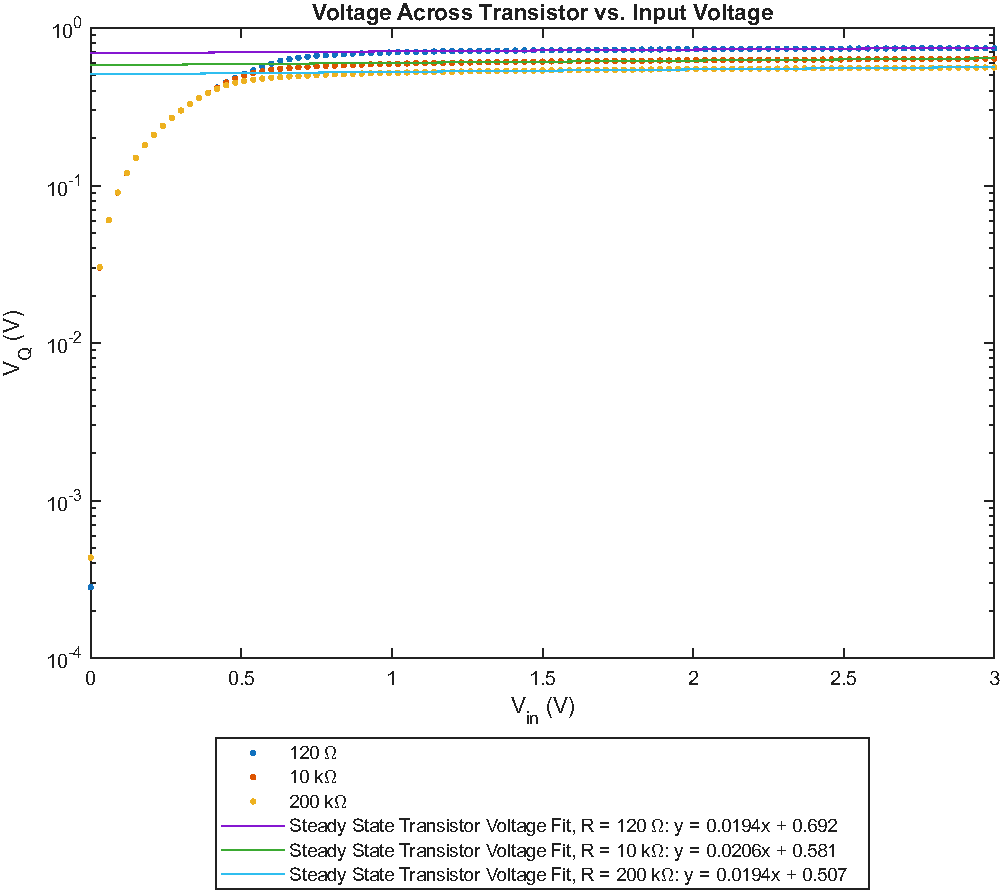
\includegraphics[width=0.7\linewidth]{../diagrams/lab2_exp2_V_in_vs_V_q.pdf}
        \caption{Voltage measured across the transistor with three different resistor values against the input voltage with best fit lines along the steady states.}\label{fig:v_in_vs_v_q}
    \end{figure}
	\subsection{Analysis}
    From the data we gathered, we observed the distinct regimes of influence in the change in voltage. For the plot with a resistance of 120 $\Omega$, we observed the current increasing linearly after the $(V_{on}, I_{on})$ point until the current outputted from the SMU limitted the linear increase. For all the other plots, this did not happen and matched our theoretical results well.
	\subsection{Discussion}
    We got 101 data points for each plot. In hindsight, this was not nearly enough measurements and contributed to the close linear approximations in the plot comparing the input voltage to the input current of the circuit. Other than that, everything else came out well and was consistent with the theoretical equations we derived from the prelab.

%----------------------------------------------------------

\end{document}